Las señales bioeléctricas y las señales de la epilepsia son temas de gran interés en la actualidad debido a su relevancia en la medicina y la neurociencia. La epilepsia es una enfermedad neurológica común que afecta a millones de personas en todo el mundo \cite{pichon2017patogenia}. La prevalencia de la enfermedad varía según el país y la región del mundo, siendo más común en niños y personas mayores, además, se estima que el 80\% de las personas con epilepsia vive en países de bajos y medianos ingresos, donde el acceso a los tratamientos puede ser limitado o inaccesible \cite{Epilepsia_OMS}.

En Guatemala, se encuentra el Centro de Epilepsia y Neurocirugía Funcional HUMANA, una organización formada por profesionales en neurociencias que trabaja con pacientes que padecen problemas neurológicos de difícil control, incluyendo la epilepsia. El centro posee el único laboratorio de vídeo electroencefalograma en Guatemala y lleva a cabo anotaciones de señales EEG manualmente, lo que implica una gran cantidad de horas de trabajo realizadas por profesionales especializados del hospital. El tiempo de operación para resaltar los segmentos de interés y finalmente dar el diagnóstico depende de la duración del registro y puede durar desde cuatro horas hasta algunos días \cite{humana_2021}. Según una entrevista realizada en 2020 al director de HUMANA, Dr. Juan Carlos Lara, las señales de donde se extraen los datos son obtenidas de personas sin y con padecimiento de epilepsias, lo que permite a los especialistas hacer las anotaciones competentes dentro de los registros \cite{camila_2022}.

En la Universidad del Valle de Guatemala (UVG) se ha estado desarrollando una herramienta de aprendizaje automático para la detección de crisis epilépticas en señales EEG. En el año 2020, María Jesús Angulo presentó un trabajo de graduación en el que se demostró que es posible detectar estas crisis mediante aprendizaje automático al caracterizar y dividir correctamente los segmentos de las señales \cite{María_ang_2020}. 

Por su parte, en el año 2021, David Alejandro Vela presentó una segunda iteración de la herramienta en su trabajo de graduación. En este caso, se realizaron ajustes a la interfaz anterior, empleando algoritmos de aprendizaje automático supervisado para clasificar la señal EEG en una de cuatro clases \cite{david_2022}. El clasificador con mejor desempeño en tiempo continuo obtuvo un promedio de exactitud del 96.7\%, utilizando máquina de vectores de soporte con características en tiempo continuo y kernel gaussiano. Además, se agregó una nueva sección a la herramienta que se encarga de la generación de anotaciones dentro de un apartado con varias opciones de personalización para la visualización. Aunque se trabajó principalmente con señales EEG en dominio del tiempo en ambas fases, se reconoce la oportunidad de analizar las señales en otros dominios y de analizar otro tipo de señales bioeléctricas. Una de las limitaciones del trabajo fue la predominancia del uso de técnicas de aprendizaje supervisado, lo que abre espacio para profundizar en el análisis de los datos con aprendizaje no supervisado. Los resultados de esta segunda fase se observan en la Figura~\ref{fig:mesh1} \cite{david_2022}. Además en la Figura~\ref{fig:app_ini} se puede ver la ventana inicial de la app y en la Figura~\ref{fig:app_chn_slct} se puede observar la forma en la que se clasifica un segmento de señal por color según su estado ictal.

\begin{figure}[t]
    \centering
    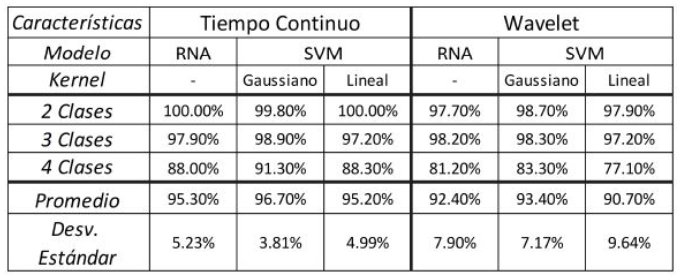
\includegraphics[width=0.5\textwidth]{figuras/David resultado.png}
    \caption{Resumen de los resultados de los clasificadores generados: red neuronal (RNN) y máquina de vectores de soporte (SVM) \cite{david_2022}.}
    \label{fig:mesh1}
\end{figure}

En el año 2022 Camila Lemus \cite{camila_2022} concluyó que las relaciones entre bandas de frecuencia son funcionales para la clasificación binaria, logrando un porcentaje de rendimiento superior al 99\% utilizando redes neuronales con dos o más características para las clases Ictal/Sano y superior a un 98.80\% para las clases Interictal/Preictal, dichos resultados se pueden observar en la Figura~\ref{fig:camila_tabla_res1}. Además, se encontró que es conveniente generar el vector de características combinando la razón 1 ($\theta/\alpha$) y la razón 2 ($\beta/\alpha$), ya que los clasificadores tienen un rendimiento igual o mayor a 98.90\% en un menor tiempo. Sin embargo, se observó que la extracción de características en dominio de la frecuencia no es muy eficiente, tardando en promedio aproximadamente 3 minutos por registro individual para procesar 409,700 muestras y 4.33 minutos para procesar 3 millones de muestras \cite{camila_2022}. El algoritmo utilizado para el análisis y el reconocimiento de patrones en señales de ECG fue \textit{K-means Clustering}. Los resultados mostraron que el algoritmo era capaz de identificar agrupaciones de señales de ECG asociadas a oscilaciones postictales de la frecuencia cardiaca. Esto sugiere que la agrupación de \textit{K-means Clustering} podría utilizarse para desarrollar un nuevo método de diagnóstico y seguimiento de la epilepsia.

\begin{figure}[t]
    \centering
    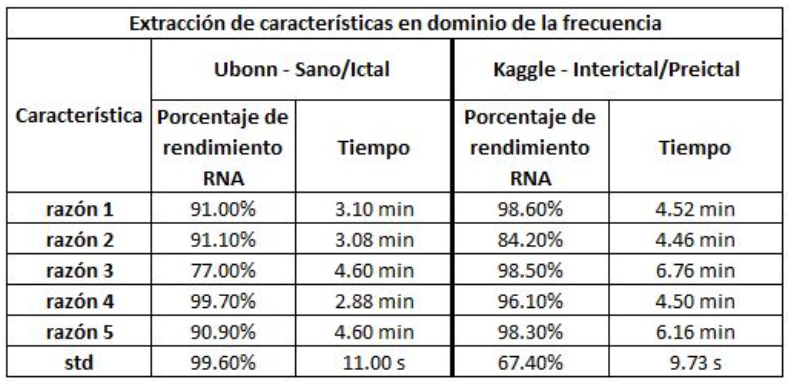
\includegraphics[width=0.5\textwidth]{figuras/3 rendimiento RNA Camila.png}
    \caption{Resumen del rendimiento de la RNN para dos clasificadores binarios utilizando características individuales en dominio de la frecuencia \cite{camila_2022}.}
    \label{fig:camila_tabla_res1}
\end{figure}

\begin{figure}[t]
    \centering
    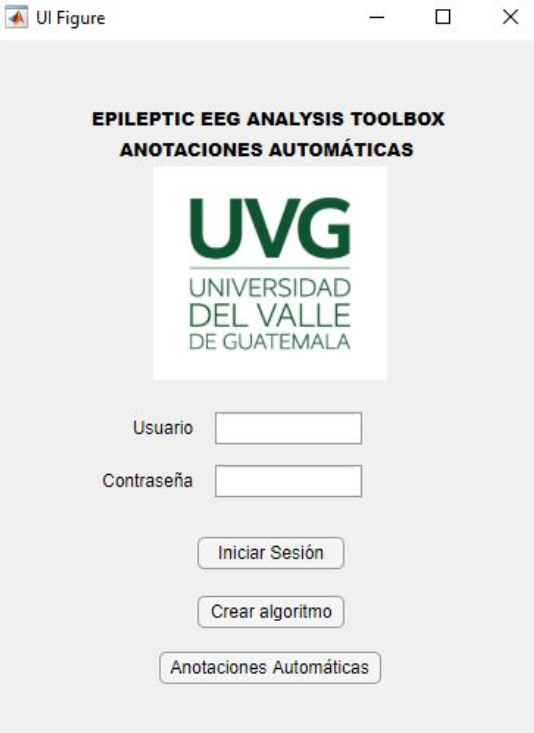
\includegraphics[width=0.5\textwidth]{figuras/4 incio app.png}
    \caption{Ventana de la aplicación para iniciar sesión \cite{david_2022}.}
    \label{fig:app_ini}
\end{figure}

\begin{figure}[ht]
    \centering
    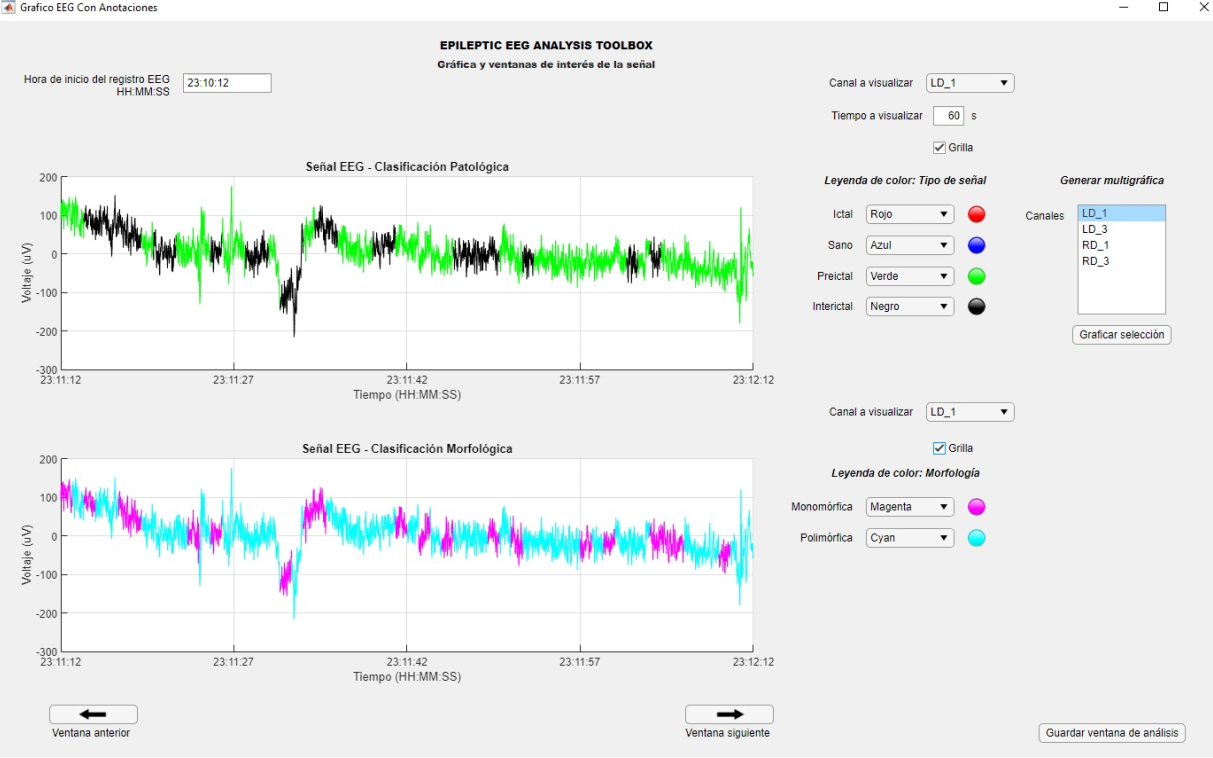
\includegraphics[width=0.5\textwidth]{figuras/5 app chn select.png}
    \caption{Ventana con la gráfica de una ventana del registro EEG del canal seleccionado \cite{david_2022}.}
    \label{fig:app_chn_slct}
\end{figure}
